% AlgoProjekt Dokumentation.
% Geschrieben in Gummi.
\documentclass[11pt]{article}
\usepackage[ngerman]{babel}
\usepackage[utf8]{inputenc}
\usepackage{graphicx}   
\usepackage{lmodern}
\usepackage{listings}
\usepackage{graphics}
\usepackage{float} 
\floatplacement{figure}{H}
\lstset{language=Java, showstringspaces=false, breaklines=true, numbers=left, frame=single, basicstyle=\tiny}
\title{\textbf{AlgoProjekt}}
\author{Maria Markstädter\\
                Noel Kuntze\\
                Ruben Anders\\}
\date{\today}
\begin{document} 

\maketitle

\newpage
\tableofcontents
\newpage
  \section{Unser Programm}
Dieses Dokument ist ein Teil des Projekts der Autoren im Rahmen ihres Studiums an der Hochschule Offenburg.
  \subsection{Programmkurzbeschreibung}
  Szenario:
Über ein Terminal wird ein Passwort eingegeben und  mittels der Hashfunktion SHA-1 verschlüsselt. Die letzten 4 Bytes (sog. Message Digest) werden über eine ungesicherte Leitung übertragen und am Authentifikationsserver mit dem Wert der für den Nutzer gespeichert wurde, verglichen. \newline 
Ziel ist es, ein gesnifftes Message Digest mit einer zuvor berechneten Hashtabelle zu vergleichen und so das Passwort herauszufinden.\vspace{2px}   \newline 
{\itshape{Dies findet in 2 Phasen statt:}} \vspace{2px}   \newline
Precomputation-Phase: Es werden Passwort und Message Digest berechnet und in einer Hashtable gespeichert.\vspace{2px} \newline 
Online-Phase: Der gesniffte Message Digest wird mit der zuvor berechneten Hashtable verglichen und so das dazugehörige Passwort herausgelesen. 
Es gilt mehrere Module zu Programmieren, die zum einen eine Hashtable erzeugen in der Passwort und Message Digest berechnet werden sowie in einer Hashtable einen zuvor gesnifften Message Digest nachschlagen und das dazugehörige Passwort ausgeben. Dies wird durch Interface unterstützt die es dem Benutzer ermöglicht einzelne Phasen anzuwählen und erstellte Hashtables zu speichern oder zu laden.

   
  \subsubsection{Programmidentifizierung}
  \paragraph{Programmname}
  AlgoProjekt
  \paragraph{Systemzuordnung des Programms}
  Kryptographie
  \paragraph{Programmversion}
  Version 1.0
  \paragraph{Freigabedatum}
  \date{26.11.2013}
  \newline
  \newline
 \subsection{Aufgabenstellung}
  Wir wollen ein einfaches, passwortbasiertes Zugangssystem angreifen. Das Zugangssystem
funktioniert wie folgt:
\begin{itemize} 
\item Der Nutzer, der sich authentifizieren will, gibt an einem gesicherten Terminal sein
Passwort ein. Der String wird mit Hilfe der kryptographischen Hashfunktion SHA-1
gehasht. Verwendet werden allerdings nur die letzten 4 Byte.
\item Das Terminal sendet diesen sogenannten Message Digest zum Authentifikationsser-
ver. Dieser vergleicht den erhaltenen Message Digest mit dem Wert, den er für die-
sen Nutzer gespeichert hat. Sind die beiden identisch, wird der Zugang freigegeben,
ansonsten nicht. 
\end{itemize}
\subsection{Funktionshierachie}
  \begin{figure}
  \centering
  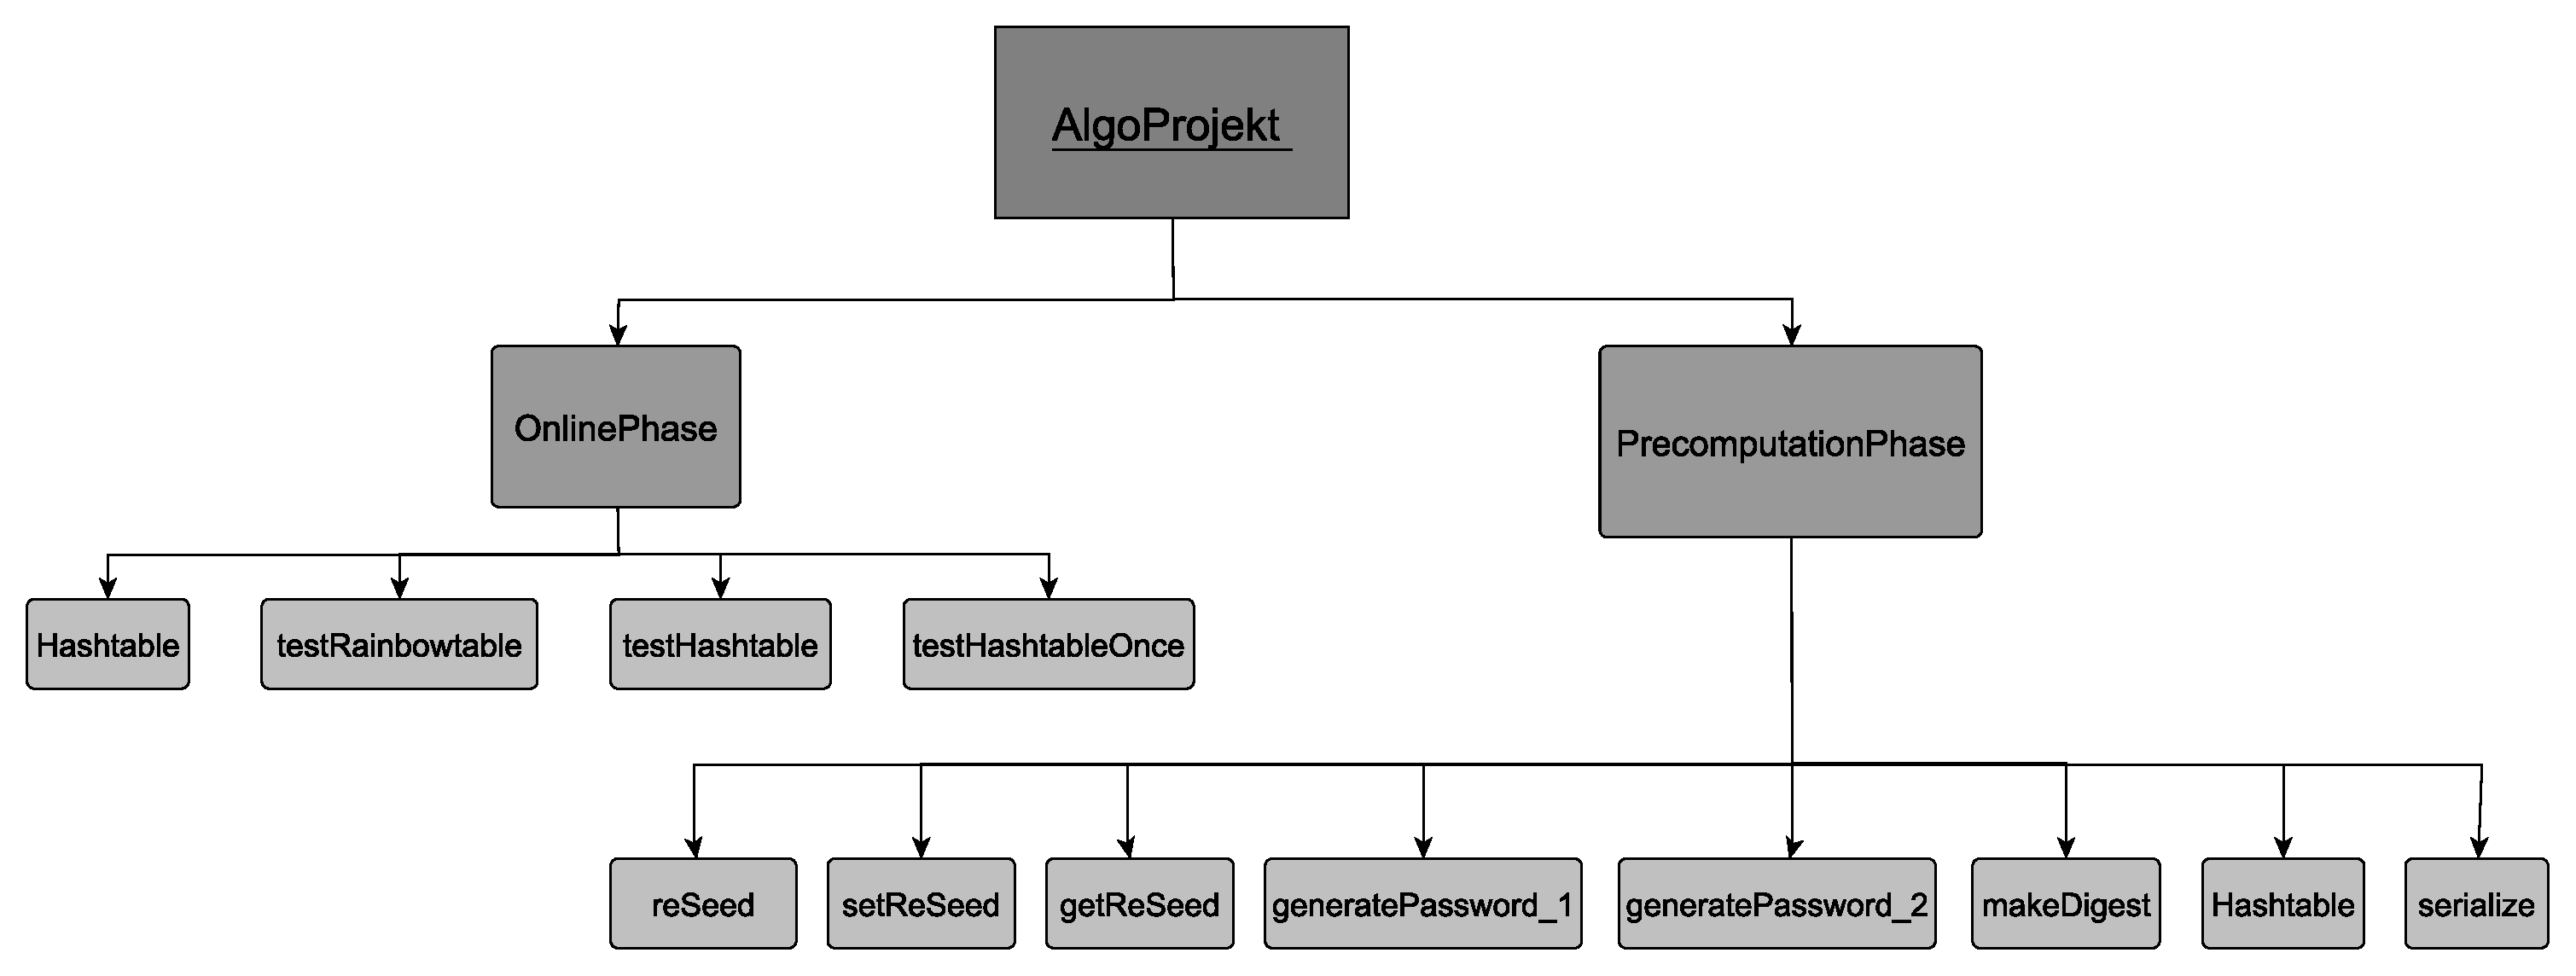
\includegraphics[width=\textwidth, clip]{Bild.pdf} 
  \caption{Klassenaufbau} 
  \end{figure} 
  \subsubsection{Methoden/Algorithmen}
  Im Programm werden verschiedene Algorithmen benutzt, um das Problem der Passwortgenerierung, Prüfsummenberechnung, Füllung der Hashtabelle, serialisierung und deserialisierung derselbigen zu lösen.
  \newline
  \pagebreak
  \begin{samepage}
  \subsubsection{Passwortgenerierung}
  Der für die Passwortgenerierung genutzte Algorithmus ist dieser: 
  \begin{lstlisting}[caption=Algorithmus zur Passwortgenerierung, label=lst:makePassword_1]
    public String generatePassword_1
    (String characters, int length) 
    {
        char[] text = new char[length];
        for (int i = 0; i < length; i++) 
        {
            if (reSeedThreshold > 0 && 
            counter == reSeedThreshold) 
            {
                this.reSeed();\centering
                counter = 0;
            }
            text[i] = characters.charAt
            (gen.nextInt(characters.length()));
            
            counter++;
        }
        return new String(text);
    }
  \end{lstlisting}
Der Input des Algorithmus besteht aus einem String, in dem die Zeichen, aus dem das Passwort bestehen soll,
und einem integer, der die Länge des Passworts angibt. Der Rückgabewert der Funktion ist ein zufälliges Passwort aus den Zeichen des Eingabestrings und der Länge des Eingabeintegers.\\
Der Algorithmus legt zuerst ein Zeichenfeld an, in das dann jeweils ein zufälliges Zeichen hineingeschrieben wird. 
Es wird ein Zeichenfeld verwendet, da das anlegen einer solchen Variable in Sachen Geschwindigkeit und Speicherplatz  billiger ist als das Anlegen eines Stringbuilders.
\\
Es existieren die Klassenattribute "reSeedThreshold", "counter", sowie "gen". Die ersten beiden Attribute sind vom Typ integer und das letzte der Klasse "Random". Die Klasse "Random"\ stellt einen Pseudozufallszahlengenerator (im Folgenden "PRNG" genannt) bereit.
\\
Das Attribut "reSeedThreshold"\ wird dazu genutzt den Pseudozufallszahlengenerator von Java nach der eingestellten Anzahl an Lesezugriffen mit einem besseren Zufallswert neu zu initialisieren. Dazu wird die Klasse
SecureRandom genutzt. Eine Instanz dieser Klasse befindet sich in der gleichen Klasse, in der auch diese Funktion ist. 
\\
Das Attribut "counter" wird bei jedem Schleifendurchlauf inkrementiert und hält so die bereits erfolgten Lesezugriffe fest. Bei jeder Neuinitialisierung wird das Attribut "counter"\ auf 0 zurückgesetzt. 
\\
Bei jedem Schleifendurchlauf wird eine Zufallszahl aus dem Zahlenraum 0 bis Länge des Eingabestrings erzeugt und das Zeichen in die entsprechenden Stelle des Strings an das Feld "text"\ eingefügt.
\\
Nach der For-Schleife wird das fertige Passwort als String von der Funktion zurückgegeben.
\\
Der PRNG wird neu initialisiert, um sicherzustellen, dass er nicht in eine Schleife gerät und wiederholt die gleiche Zahlenfolge ausgibt, was zu sich wiederholenden Passwörtern führen würde
Das Reinitialisieren kann man durch das setzen des Werts "reSeedThreshold"\ auf "0" deaktivieren.
\end{samepage}
\subsubsection{Prüfsummenberechnung}
Für die Prüfsummenberechnung wird dieser Algorithmus genutzt: 
\begin{samepage}
\begin{lstlisting}[caption=Algorithmus zur Prüfsummenberechnung, label=lst:makeDigest]
    public static String makeDigest(String passwd, 
    String algorithm) 
    {
        byte digest[];
        byte shortenedDigest[] = new byte[4];
        int i;
        MessageDigest md;
        
        try {
            md = MessageDigest.getInstance(algorithm);
        } catch (NoSuchAlgorithmException e) {
            System.err.println(
            "Sorry, Java doesn't know that algorithm: "
             + algorithm);
            e.printStackTrace();
            return null;
        }
        
        digest = md.digest(passwd.getBytes());
        
        /* We only need the first 32 bit 
         * (the first 4 byte), so we copy the
         * last 4 bytes to our own array
         */
        for (i = 0; i < 4; i++) {
            shortenedDigest[i] = digest[digest.length - 4 + i];
        }
        
        /* We need to translate the bytes 
         * to hexadecimal strings, because HashMaps
         * and Hashtables use object.equals 
         * to find matching objects
         * in the table, which a byte array doesn't provide.
         */
         
        StringBuffer sb = new StringBuffer();
        
        /* Transform the byte array into a hexadecimal string */
        
        for (i = 0; i < shortenedDigest.length; i++) {
            sb.append(integer.toString((shortenedDigest[i] & 0xff) 
            + 0x100, 16).substring(1));
        }
        
        return sb.toString();

    }
\end{lstlisting}
\end{samepage}
Der Funktion werden das Passwort und der zu verwendende Algorithmus in Stringform übergeben.
Der Rückgabewert der Methode ist eine auf 32-Bit abgeschnittene Prüfsumme des Eingabestrings unter Verwendung des angegebenen Algorithmus.\\
Zuerst werden die benötigten Variablen deklariert. Das sind zwei Byte-Arrays für die Digests, sowie ein integer als Zählvariable der Zählschleife. Desweiteren wird ein Objekt der Klasse MessageDigest benötigt, um den Hash des Passworts zu berechnen. \\
Im nächsten Schritt wird versucht eine Instanz des Prüfsummenalgorithmus zu erstellen. Falls das fehlschlägt, wird eine entsprechende Fehlermeldung, sowie ein StackTrace ausgegeben und die Funktion liefert "null"\ zurück.\\
Danach wird der Digest des Passworts mit "md.digest(passwd.getBytes())"\ berechnet und in einen StringBuffer geschrieben. Der StringBuffer wird benötigt, da Strings in Java nicht veränderbar sind. Das wird umgangen, indem man StringBuilder oder StringBuffer verwendet. \\
Im darauf folgenden Schritt werden die letzten 4 Byte des Digest in ein anderes Feld kopiert, welches dann in Hexadezimalschreibweise in einen String geschrieben wird. Das ist nötig, da die Methode "get" der Hashtables und Hashmaps in Java die Methode "\ equals"des Eingabeobjekts benutzen, um die Eingabeobjekte mit den Objekten in der Tabelle zu vergleichen. Ein Bytearray besitzt diese Methode jedoch nicht, weshalb das Suchen in einer Hashtabelle damit nicht funktionieren würde.
Im letzten Schritt wird der Inhalt des StringBuffers, der im Moment den Digest darstellt, in einem String umgewandelt und zurückgegeben.\\
In der Methode werden überwiegend Primitivtypen benutzt, da diese schneller anzulegen sind und einen geringeren Speicherplatzbedarf haben im Vergleich mit komplexen Klassen.


\subsubsection{Speicherung}
\begin{lstlisting}[caption=Algorithmus zur Füllung der Hashtabelle, label=lst:makeTable]
    public Hashtable<String, String> 
    makeTable(int amount, String legalChars, int length) {
        int i;
        String password;
        float time1, time2;
        Hashtable<String, String> table = 
        new Hashtable<String, String>(amount,95);
        System.out.println("Generating " + 
        amount + " hash table entries ...");
        time1 = System.currentTimeMillis();
        for (i = 0; i < amount; i++) {
            password = generatePassword_1
            (legalChars, length);
            table.put(makeDigest
            (password, "SHA-1"), password);
        }
        time2 = System.currentTimeMillis();
        System.out.println("Generating the hash table entries took " 
        + (time2 - time1) + " ms.");
        System.out.println("The table now holds " + table.size() 
        + " entries.");
        return table;
    }
\end{lstlisting}
Die Methode zur Erstellung einer Hashtabelle lässt sich mit 3 Parametern steuern. Diese sind die Menge an Einträgen, die erstellt werden sollen, die Zeichen, aus denen die Passwörter generiert werden sollen, sowie die Länge der Passwörter.\\
Die Funktion liefert eine Hashtabelle mit dem gewünschten Inhalt zurück.
Zuerst werden einige Variablen deklariert. Darunter sind eine Zählvariable i, eine Stringreferenz für das jeweilig generierte Passwort für den Eintrag, zwei floats um die Zeit zu messen, die die Generierung der Tabelle benötigt und eine Hashtabelle, die Strings zu Strings mapt und die entsprechende Größe für die benötigte Menge an Einträgen hat. Das vermeidet das bewegen der Tabelle im Speicher, sobald sie über den Schwellwert hinaus anwächst.\\
Danach wird eine Meldung für den Benutzer ausgegeben, wieviele Einträge erstellt werden.
Nun wird die Tabelle mit der entsprechenden Anzahl an Digest-Passwort-Toupeln befüllt. Dazu wird die Methode makeDigest() genutzt.\\
Für die Zeitmessung wird die Systemzeit vor und nach dem Befüllen der Tabelle festgehalten und die Differenz ermittelt. Die Differenz wird dann an den Benutzer ausgegeben. Am Ende der Methode wird die Anzahl der Einträge in der Tabelle ausgegeben. Daraus kann man die Anzahl an Hash-Kollisionen beim Befüllen der Tabelle berechnen.
\\Der letzte Schritt ist die Rückgabe der Tabelle.
\begin{lstlisting}[caption=Algorithmus zur Serialisierung der Hashtabelle, label=lst:serializing]
    public static void serialize(Hashtable
    <String, String> table, String path) {
        System.out.println(
        "Please wait while the file is being created."
        );
        FileOutputStream f_out = null;
        File file = new File(path);
        try {
            file.createNewFile();
        } catch (IOException IOEx) {
            System.out.println(
            "Something bad happened!"
            );
            System.out.println("Stacktrace:");
            IOEx.printStackTrace();
        }
        if (!file.canWrite()) {
            System.out.println(
            "Can't write to the file. Aborting."
            );
        }
        try {
            f_out = new FileOutputStream(path);
        } catch (FileNotFoundException e) {
            System.out.println("File not found!");
        }
        ObjectOutputStream obj_out = null;
        try {
            obj_out = new ObjectOutputStream(f_out);
        } catch (IOException | NullPointerException e) {
            System.out.println("Something bad happened!");
            System.out.println("Stacktrace:");
            e.printStackTrace();
        }
        //Schreibt das Aray in eine Datei
        try {
            obj_out.writeObject(table);
        } catch (IOException | NullPointerException e) {
            System.out.println(
            "Couldn't write the hash table to the file!"
            );
        }
    }
\end{lstlisting}
Diese prozedur serialisiert eine gegebene Hashtabelle und speichert sie im gegebenen Pfad.\\
Zuerst wird eine Meldung für den Benutzer ausgegeben, damit er weiß, dass der Prozess läuft und das Programm arbeitet. Dann wird eine Datei erstellt und auf mögliche Fehler überprüft. Im darauf folgenden Schritt wird versucht das Objekt in die Datei zu schreiben. Überprüfungen der Pfadangabe verhindern, dass ungültige Pfade oder Pfade zu Verzeichnissen der Prozedur übergeben werden. Diese Überprüfungen sind im Code vor dem Aufruf dieser Prozedur untergebracht. 
\pagebreak
\begin{lstlisting}[caption=Algorithmus zur Deserialisierung einer Datei und Einlesen einer Hashtabelle, label=lst:deserializing]
    public static Hashtable<String, String> 
    deserialize(String filename) {
        Hashtable<String, String> table = 
        new Hashtable<String, String>();

        System.out.println(                
        "Trying to load the hash table from \"" + filename + "\"..."
        );
        FileInputStream f_in = null;
        try {
            f_in = new FileInputStream(filename);
        } catch (FileNotFoundException ex) {
            System.out.println(
            "The specified file to load doesn't doesn't exist!"
            );
        }
        ObjectInputStream obj_in = null;
        try {
            obj_in = new ObjectInputStream(f_in);
        } catch (IOException ex) {
            System.out.println(
            "Couldn't create the ObjectInputStream " +
            "needed to load the Object from the file!"
            );
            return null;
        }
        System.out.println("Loading ...");
        /* We try to read the object from the file */
        try {
            table = (Hashtable<String, String>) 
            obj_in.readObject();
        } catch (IOException IOex) {
            System.out.println(
            "Something bad happened while " +
            "accessing the specified file!"
            );
            return null;
        } catch (ClassNotFoundException CNF) {
            System.out.println(
            "The specified file to load doesn't " +
             "contain an apropriate object!"
            );
            return null;
        }

        if (table != null) {
            System.out.println(
            "The file \"" + filename + 
            "\" was successfully loaded."
            );
        }
        try {
            obj_in.close();
        } catch (IOException ex) {
            System.out.println(
            "Couldn't close the ObjectInputStream!"
            );
            System.out.println("Stacktrace:");
            ex.printStackTrace();
        }
        try {
            f_in.close();
        } catch (IOException ex) {
            System.out.println(
            "Couldn't close the FileInputStream!"
            );
            System.out.println("Stacktrace:");
            ex.printStackTrace();
        }
        return table;
    }
\end{lstlisting}

Diese Funktion liest eine Hashtabelle aus einem angegebenen Pfad ein und gibt eine Referenz zum eingelesenen Objekt zurück.\\
Im Code wird versucht einen FileInputStream von der Datei zu erstellen, sodass im Folgenden ein ObjectInputStream erstellt werden kann. Danach wird die Hashtabelle mit dem ObjectInputStream aus der Datei ausgelesen. Am Ende der Funktion werden die InputStreams geschlossen. Während des gesamten Vorgangs werden Ausnahmefehler abgefangen und behandelt.
  \subsection{Programmbausteine}
  \subsubsection{Klasse Algoprojekt}

  \textbf{Variablen in der Main-Funktion}\\
  \begin{tabular}{rlr}
  Variablenname & Typ & Standardwert \\
  length & int & 6 \\
  reSeed & int & 150000 \\
  i & int & nicht initialisiert \\
  value & int & nicht initialisiert \\
  generateOnly & boolean & false \\
  interactive & boolean & false \\
  isInteger & boolean & false \\
  wrong\_option & boolean & true \\
  accepted & boolean & false \\
  
  \end{tabular}\\
  \textbf{Objekte in der Main-Funktion}\\
  \begin{tabular}{rlr}
  Variablenname & Klasse & Standardwert \\
    loadTablePath & String & null \\
  storeTablePath & String & null \\
  legalChars & String & \{A-Z,a-z,0-9,Sonderzeichen\} \\
  password & String & null \\
  amount & String & 10000000 \\
  path & String & Nicht zutreffend \\
  option & String & null \\
  result & String & null \\
  pathdescriptor & File & Nicht zutreffend\\
  Ne & NumberFormatException & Nicht zutreffend \\
  IOEx & IOException & Nicht zutreffend \\
  phase & PrecomputationPhase & Nicht zutreffend \\
  table & Hashtable String, String & Nicht zutreffend \\
  isr & InputStreamReader & Nicht zutreffend \\
  br & BufferedReader & Nicht zutreffend \\
  
  \end{tabular}
  \subsection{Fehlerbehandlung}
  \subsubsection{Dateipfade}
  \paragraph{Zu lesende Dateien:} 
  Jede Benutzereingabe wird im Programm auf Plausabilität getestet. 
  Unter anderem werden Dateipfade auf Zugänglichkeit, sowie Lesefähigkeit und Existenz geprüft.\\
\begin{samepage}
  \textbf{Codebeispiel}
\begin{lstlisting}[caption=Überprüfung eines Eingabedateipfads, label=lst:InputPathValidation]
accepted = false;
while (!accepted) {
        accepted = true;
    System.out.println("Please enter the path to the file: ");
    try {
    path = br.readLine();
    } catch (IOException IOex) {
            System.err.println(
            "Sorry, couldn't read the path" + 
            " from the terminal!\n"
            );
            System.err.println("Stacktrace:");
            IOex.printStackTrace(System.err);
            return;
    }
    pathdescriptor = new File(path);
    if (!pathdescriptor.exists()) {
            System.err.println(
            "The specified file doesn't exist!"
            );
            accepted = false;
    }
    if (!pathdescriptor.canRead()) {
                System.err.println("The specified file can't be read!");
    }
    if (!pathdescriptor.isFile()) {
            System.err.println(
            "The specified path doesn't point to a file!"
            );
             accepted = false;
     }
}
table = deserialize(path);
\end{lstlisting}
\end{samepage}
\pagebreak
\begin{samepage}
  \paragraph{Zu schreibende Dateien:}
Bei zu schreibenden Dateien ist die Fehlerüberprüfung sehr eingeschränkt, da Dateioperationen nur ausgeführt werden sollten, wenn sicher ist, dass sie auch erfolgreich abgeschlossen werden können. Daher wird hier nur darauf geprüft, ob die zu schreibende bereits Datei existiert.
  \begin{lstlisting}[caption=Überprüfung eines Ausgabedateipfads, label=lst:OutputPathValidation]
                          while (!accepted) {
                            accepted = true;
                            System.out.print("Please enter a path: ");
                    try {
                        path = br.readLine();
                    } catch (IOException IOEx) {
                        System.err.println("Sorry, couldn't read the path from the terminal!");
                        System.err.println("Stacktrace:");
                        IOEx.printStackTrace(System.err);
                    }
                            path += ".ser";
                            pathdescriptor = new File(path);
                            System.out.println("Saving in \"" + path + "\"");
                            if (pathdescriptor.exists()) {
                                System.err.println("The specified file already exists");
                                accepted = false;
                            }
                        }
                        serialize(table, path);
  \end{lstlisting}
  \end{samepage}
  \pagebreak
  \subsubsection{Zahleneingaben}
Analog werden auch Zahleneingaben des Nutzers überprüft und der Nutzer davon abgehalten Aktionen auszuführen, die im Momentanen Zustand des Programms nicht möglich sind, zum Beispiel das Suchen von Passwörtern in der Hashtable, wenn keine Hashtable geladen ist.
 Falls der Nutzer es trotzdem versucht, gibt das Programm eine Fehlermeldung aus und der Benutzer hat die Möglichkeit eine neue Option zu wählen.
Im ausgewählten Quellcodeausschnitt sind die Optionen Vier, Fünf und Sechs nur verfügbar, wenn auch eine Tabelle geladen wurde, die Referenz "table\"\ also ungleich Null ist. Da der Zahlenraum der verfügbaren Optionen im Bereich zwischen eins und 7 ist, werden nur Zahlen größer Null und kleiner gleich Sieben akzeptiert.\\
\begin{lstlisting}[caption=Überprüfung von Zahlen, label=lst:checkIntegers]
while (wrong_option || !isInteger || value == 0) {
  /* We try to read a line from the buffered reader. */
        try {
                option = br.readLine();
        } catch (IOException ex) {
                System.err.println(
                "We couldn't read from the terminal. Sorry :("
                );
                System.err.println("Stacktrace:");
                ex.getStackTrace();
                return;
        }
    /* We try to  parse the input line as an integer */
    try {
            value = Integer.parseInt(option);
    } catch (NumberFormatException NFe) {
            System.err.println("Please enter a valid integer.");
        isInteger = false;
    } finally {
                /* We check for the range of options, 
                 * so you can't enter -1 or 8. 
                 */
                if (value > 0 && value <= 7) {
                        isInteger = true;
            }
           }
   /* This checks if the value chosen 
    * from the user is applicable to 
    * the current state of the program.
    * E.g.: Whether a hashtable was loaded or not 
    */
    if ((value == 3 || value == 4 || value == 5 || value == 6) 
    && table == null) {
            System.err.println(
            "Load a hash table before you try to use those!"
            );
            wrong_option = true;
        } else {
            wrong_option = false;
    }
}
  \end{lstlisting}
  \subsubsection{Programmparameter}
  Da dem Programm Parameter übergeben werden können ist es wichtig, diese auch zu überprüfen, um ein Fehlverhalten des Programms auszuschließen. Das Programm versteht Parameter, die Pfade sind, als auch Zahlen
  , Zeichenketten und einfache Switches, daher existieren auch verschiedene Wege diese zu überprüfen.
  Um den Codeausschnitt nicht unnötig aufzublähen, wurde nur jeweils ein Parameter jeden Typs ausgewählt.
  Im Codeausschnitt werden die Parameter in einer FOR-Schleife verarbeitet.\\
  Bei Eingabedateiparametern sollte beim Programmstart bereits überprüft werden, ob die Zieldatei existiert, lesbar ist und nicht ein Verzeichnis o.Ä. ist. Das wird in der Verarbeitung des Parameters "\---file" deutlich.\\
 Für Ausgabedateiparameter kann zum Zeitpunkt der Parameterprüfung nur überprüft werden, ob eine solche Datei bereits existiert. Andere Überprüfungen würden eigentliche Schreiboperationen und das Anlegen einer Datei benötigen, was jedoch zu diesem frühen Zeitpunkt zu vermeiden ist.\\
Bei Zahlenparametern muss direkt bei der Verarbeitung geprüft werden, ob der angegebene Parameterwert auch als Zahl interpretierbar ist.\\
Bei allen Parametertypen, außer Switches, ist es nötig die Zählvariable zu inkrementieren, denn sonst würde beim nächsten Durchlauf der FOR-Schleife versucht werden, den Parameterwert als Parameter zu interpretieren.
Die Beispiele für diese verschiedenen Typen sind hier der Fall "\---file" für Eingabedateiparameter, der Fall "\--output" für Ausgabedateiparameter, der Fall "\---generate" für Switches, sowie der Fall "\---number" für Zahlenvariablen.
\begin{lstlisting}[caption=Überprüfung der Programmparameter, label=lst:checkParameter]
for (i = 0; i < args.length; i++) {
        switch (args[i]) {
        
                case "--help":
                        printHelpMessage();
                        return;
                        
           case "--file":
                if (i < args.length - 1) {
                            String path = args[i + 1];
                            File pathdescriptor = new File(path);
                    if (!pathdescriptor.exists()) {
                            System.out.println(
                            "The specified file for the --file option doesn't exist!"
                            );
                                return;
                        }
                        if (!pathdescriptor.canRead()) {
                                System.out.println(
                                "The specified file for the --file option can't be read!"
                                );
                                return;
                        }
                        if (!pathdescriptor.isFile()) {
                                System.out.println(
                                "The specified path doesn't point to a file!"
                                );
                                return;
                        }
                                 loadTablePath = path;
                                i++;
                } else {
                                System.out.println(
                                "Using the --file option requires a file after it!"
                                );
                                return;
                        }
                break;


        case "--output":
        
    if (i < args.length - 1) {
            String path = args[i + 1];
            File pathdescriptor = new File(path + ".ser");
            System.out.println("Saving in \"" + path + "\"");
            if (pathdescriptor.exists()) {
                    System.out.println(
                    "The specified file for the --output option already exists!"
                    );
                    return;
            }
            storeTablePath = path;
        i++;
        } else {
        System.out.println("Using the --output option requires a file after it!");
                return;
                }
                break;

        case "--generate":
                generateOnly = true;
                break;
                
        case "--number":
                if (i < args.length - 1) {
                        try {
                                amount = Integer.parseInt(args[i + 1]);
                                } catch (NumberFormatException Ne) {
                                        System.err.println(
                                        "Using the --number option requires an integer after it!"
                                        );
                                        return;
                } finally {
                        i++;
                        }
                        
                } else {
                        System.err.println(
                        "Using the --number option requires an integer after it!"
                        );
                        return;
                }
                break;
        default:
                System.err.println(
                "Option " + args[i] + " isn't known!"
                );
        return;
        }
}
\end{lstlisting}
  
   \section{Programmtest}
  \subsection{Testziele}
  Die Testziele sind das Sicherstellen der Funktionalität des Programms und des sicheren Ablaufs desselbigen.
  
  \subsection{Testverfahren}
Die Entwicklungsumgebung wird genutzt, um das Programm mit verschiedenen Parameterkombinationen zu starten. Der Tester überprüft dann die Funktionalität des Programms und vergleicht das Verhalten des Programms mit seinem Erwartungen and das Verhalten desselbigen.
  \subsection{Testfälle/Testresultate}
  \subsubsection{Testfall 1: Generieren und Speichern der Hashtabelle}
    In diesem Testfall soll die Hashtable generiert und gespeichert werden. Dazu wird das Programm mit den Parametern "-g -o test.ser" aufgerufen. Das Programm generiert dadurch eine Hashtabelle mit den Standardeinstellungen und speichert sie im Arbeitsverzeichnis in die Datei "test.ser".\\
    \textbf{Programmaufruf:} "java -jar AlgoProjekt.jar -g -o test.ser"\\
    \textbf{Programmausgabe:}
    \begin{verbatim}
Saving in "test.ser"
Generating 10000000 hash table entries ...
Generating the hash table entries took 5784.0 ms.
The table now holds 9877523 entries.
Please wait while the file is being created.
    \end{verbatim}
    \textbf{Überprüfung der erstellten Datei:}\\
    Hierzu wird die Datei mit dem Programm geladen. Siehe Test 2.\\
    \textbf{Programmaufruf:}
    "java -jar AlgoProjekt.jar -f test.ser"\\
         \textbf{Programmausgabe:}
         \begin{verbatim}
Trying to load the hash table from "test.ser"...
Loading ...
The file "test.ser" was successfully loaded.
Please enter the password you want to search for: 
asfasf
Sorry, no matching entry in the table.
         \end{verbatim}
         Nach der Zeile "Please enter the password you want to search for:"\
         muss ein String eingegeben werden, damit das Programm weiterläuft.\\
         \textbf{Erwartetes Testresultat:}\\
Das Programm erstellt und speichert eine Hashtabelle in der Datei "test.ser"\ im Arbeitsverzeichnis.\\
\textbf{Erzieltes Testresultat:}\\
Die Datei wurde erstellt und das anschließende Laden der Datei zeigt auch, dass eine Hashtabelle in ihr enthalten ist.
\subsubsection{Testfall 2: Laden und nutzen einer Hashtabelle}
In diesem Testfall soll eine Hashtabelle aus einer Datei geladen und interaktiv im Programm genutzt werden. Dazu wird das Programm mit den Parametern "\ -f test.ser -i"\ ausgeführt.\\
\textbf{Programmaufruf:} java -jar AlgoProjekt.jar -f test.ser -i \\
\begin{samepage}
\textbf{Programmausgabe:}
\begin{verbatim}
Trying to load the hash table from "test.ser"...
Loading ...
The file "test.ser" was successfully loaded.
Please choose an option:
1 - Create a new hash table.
2 - Load a hash table.
3 - Save the hash table.
4 - Look up a password in the hash table.
5 - Generate a password and look it up in the hash table.
6 - Test the hash table with a number of generated passwords.
7 - Quit.
\end{verbatim}
\end{samepage}
Nach dem Ende der Ausgabe muss das Programm mit \begin{verbatim}4 
axr?AK 
\end{verbatim} 
angewiesen werden in der Hashtabelle nach dem Digest des Strings axr?AK zu suchen.\\
\textbf{Programmeingabe:}
\begin{verbatim}
4
axr?AK
\end{verbatim}
\textbf{Programmausgabe:}
\begin{verbatim} 
Enter a password:
axr?AK
A password with the same hash value has been found: )aQ$LU
Please choose an option:
1 - Create a new hash table.
2 - Load a hash table.
3 - Save the hash table.
4 - Look up a password in the hash table.
5 - Generate a password and look it up in the hash table.
6 - Test the hash table with a number of generated passwords.
7 - Quit.
\end{verbatim}
\textbf{Erwartetes Testresultat:}\\
Das auffinden einer Kollision und keine Ausgabe einer Fehlermeldung.\\
\textbf{Erzieltes Testresultat:}\\
Das Auffinden einer Kollision und keine Fehlermeldung.
\newpage
\section{Verbesserungsvorschläge}
\begin{itemize}
\item Es ist von Vorteil, wenn das Programm selbst erkennt, dass der Heap-Space für die zu generierende Anzahl an Einträgen nicht ausreichen wird und das dem Nutzer meldet.
\end{itemize}
\end{document}
